\documentclass[10pt,a4paper]{ieeetran}
\usepackage[latin1]{inputenc}
\usepackage{amsmath}
\usepackage{amsfonts}
\usepackage{amssymb}
\usepackage{graphicx}
\usepackage{float}
\usepackage{gensymb}
\usepackage{hyperref}
\usepackage{cite}
\usepackage[justification=centering, font={small,it}]{caption}
\author{Dicson Wijaya (1002289), Wenkie Lau (1002219), \\ Mok Jun Neng (1002219), Charlotte Phang (1002277),\\ Martin Tan (1002173)}
\title{Physical World 2D Report}
\begin{document}
	\maketitle
	\section{Methodology}
	 The following methodology was used to find $\lambda_{algae bottle}$:\\
	 \begin{enumerate}
	 	\item Fill the bottle with 30ml of hot water at $50 \degree C$ to $60 \degree C$
	 	\item Place thermocouples in the bottle and the tank
	 	\item 
	 \end{enumerate}
 	
 	\section{Design of Heat Exchanger}
 	
 	\section{Demonstration}
 		\begin{figure}[H]
 			\begin{center}
 				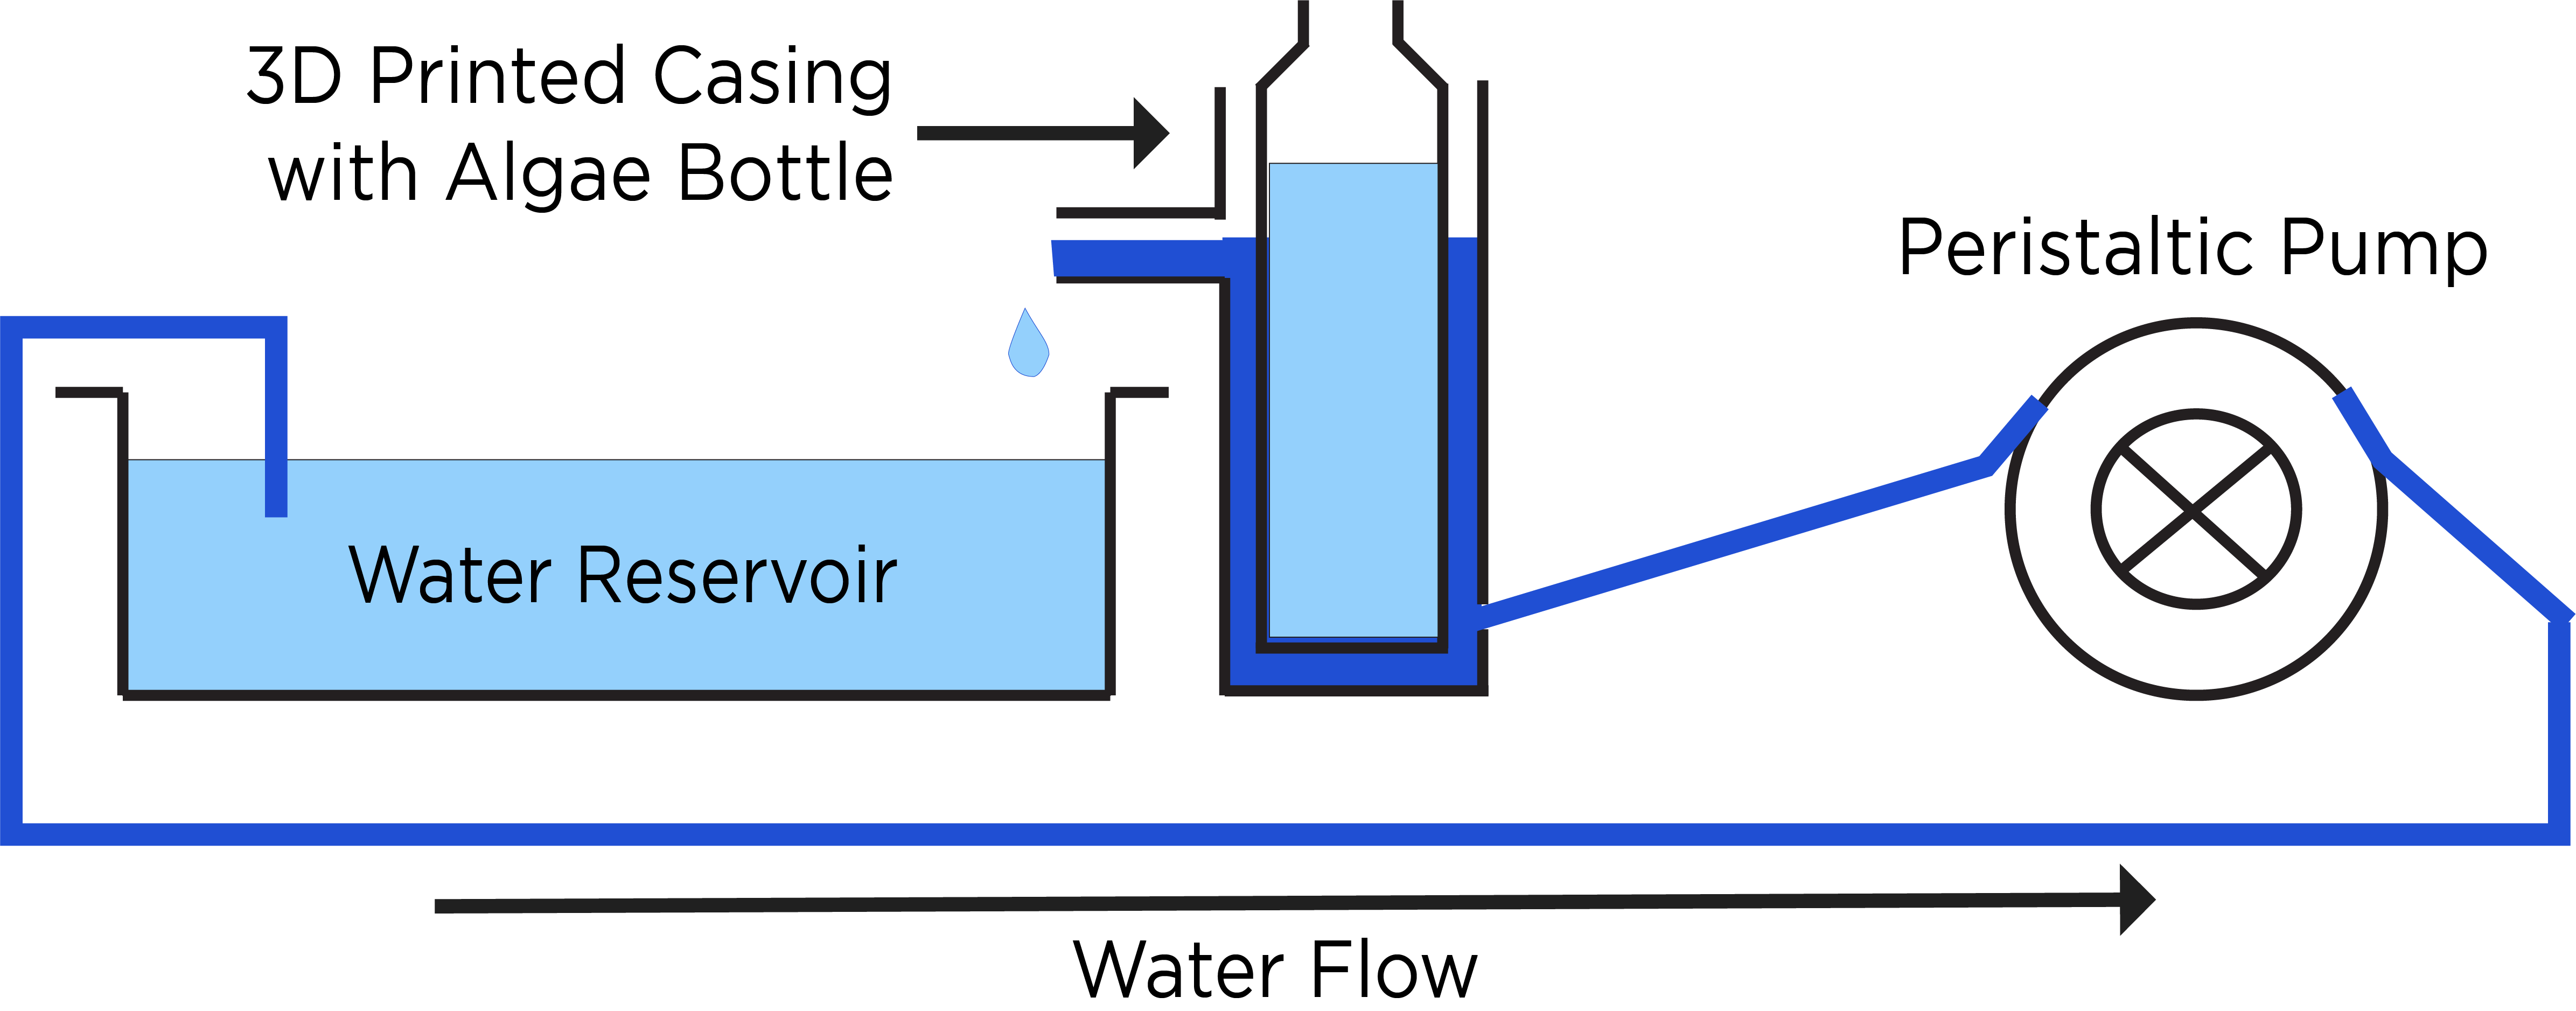
\includegraphics[width=0.5\textwidth]{demo_setup.png}
 				\caption{}
 				\label{fig:demo_setup}
 			\end{center}
 		\end{figure}
	 
	\section{Wcv}
	\begin{enumerate}
		\def\labelenumi{\roman{enumi}.}
		\item The equation of control volume in the heat exchanger
		$$\frac{dE_{cv}}{dt} = \dot{Q}_{cv} - \dot{W}_{cv} + \dot{m}_{i} \left( h_i + \frac{V_i}{2} + gz_i \right) + \dot{m}_{e} \left( h_e + \frac{V_e}{2} + gz_e \right)$$ \\
		\textit{Assume steady state, so $\dot{m}_{i} = \dot{m}_{e} = \frac{dE_{cv}}{dt} = \dot{m}$ No change in potential and kinetic energy} \\
		\textit{Air is ideal gas.} \\
		$$\frac{dE_{cv}}{dt} = \dot{Q}_{cv} - \dot{W}_{cv} + \dot{m} \left( h_1 - h_2 \right)$$ \\
		\item The rate of heat entering control volume \\
		$$\dot{Q}_{cv} = \dot{Q}_{exchanged}$$ \\
		$$\dot{Q}_{cv} = m_a c_a \left( \frac{dT_a}{dt} \right) - \dot{Q}_{ambient}$$ \\
		$$\dot{Q}_{cv} = m_a c_a \left( \frac{dT_a}{dt} \right) - \lambda_{algaebottle} \left( T_a - T_{amb} \right)$$ \\
		\textit{By substituting value of $\lambda_{algaebottle} = 1.76$} \\
		$$\dot{Q}_{cv} = m_a c_a \left( \frac{dT_a}{dt} \right) - 1.76 \left( T_a - T_{amb} \right)$$ \\
		\item The equation of control volume in the heat exchanger \\
		\textit{From simplified $\frac{dE_{cv}}{dt}$ equation in the previous part} \\
		$$\frac{dE_{cv}}{dt} = \dot{Q}_{cv} - \dot{W}_{cv} + \dot{m} \left( h_1 - h_2 \right)$$ \\
		\item Express $\dot{W}_{cv}\ = f \left( T_a \right)$ assuming $\dot{W}_{cv}$ is a constant
		\textit{Assume that $\frac{dE_{cv}}{dt} = 0$} \\
		$$0 = m_a c_a \left( \frac{dT_a}{dt} \right) - \lambda_{algaebottle} \left( T_a - T_{amb} \right) - \dot{W}_{cv} + \dot{m} \lbrack c_w \left( T_i - T_e \right) \rbrack$$ \\
		$$\lambda_{algaebottle} \left( T_a - T_{amb} \right) + \dot{W}_{cv} - \dot{m} \lbrack c_w \left( T_i - T_e \right) \rbrack = m_a c_a \left( \frac{dT_a}{dt} \right)$$ \\
		$$\int 1 dt = \int \frac{m_a c_a}{\lambda_{algaebottle} \left( T_a - T_{amb} \right) + \dot{W}_{cv} - \dot{m} \lbrack c_w \left( T_i - T_e \right) \rbrack} dT_a$$ \\
		$$t+ c = \frac{m_a c_a}{\lambda_{algaebottle}} \ln(\lambda_{algaebottle} \left( T_a - T_{amb} \right) + \dot{W}_{cv} - \dot{m} \lbrack c_w \left( T_i - T_e \right) \rbrack)$$ \\
		$$\frac{\lambda_{algaebottle} \left( t + c \right)}{m_a c_a} = \ln(\lambda_{algaebottle} \left( T_a - T_{amb} \right) + \dot{W}_{cv} - \dot{m} \lbrack c_w \left( T_i - T_e \right) \rbrack)$$ \\
		$$e^{\frac{\lambda_{algaebottle} \left( t + c \right)}{m_a c_a}} = \lambda_{algaebottle} \left( T_a - T_{amb} \right) + \dot{W}_{cv} - \dot{m} \lbrack c_w \left( T_i - T_e \right) \rbrack$$ \\
		$$\dot{W}_{cv} = e^{\frac{\lambda_{algaebottle} \left( t + c \right)}{m_a c_a}} - \lambda_{algaebottle} \left( T_a - T_{amb} \right) + \dot{m} \lbrack c_w \left( T_i - T_e \right) \rbrack$$
	\end{enumerate}
	
	\section{Derivation}
	$$T_i - T_{amb} = -R \rho V c \frac{dT}{dt}$$
	$$\int_{0}^{t} dt = -R \rho V c \int_{T_i}^{T}\frac{1}{T-T_{amb}} dT$$
	$$\frac{t}{R \rho V c} = \ln \left| \frac{T - T_{amb}}{T_i - T_{amb}} \right|$$
	$$\left( T_i - T_{amb} \right) e^{-\frac{t}{R \rho V c}} = T - T_{amb}$$
	$$\Delta T = \Delta T_{initial} e^{-\frac{t}{R \rho V c}}$$
	
	\bibliography{final_report}
	\bibliographystyle{ieeetr}
\end{document}